\documentclass[a4paper,11pt]{article} %Selecionando a classe que gera artigos.

%PACOTES ABNT
\usepackage[brazil]{babel} % Pacote para usar portugues.
%Babel traduz como “table of contents“, “chapter” e “section“, sejam impressas como “sumário”, “capítulo” e “seção”, respectivamente.

\usepackage[T1]{fontenc} %Pacote para copiar palavras com acentuação do pdf de um documento feito em LaTeX que tenha usado esses pacotes resultará nas palavras corretamente acentuadas

\usepackage[utf8]{inputenc} % Pacote para poder usar acentuação no arquivo .tex

%\usepackage{biblatex}


\usepackage{graphicx} %Pacote para inserir Figuras.

\usepackage[top=2.0cm,right=2.0cm,left=2.0cm,bottom=2.0cm]{geometry} %Pacote de Margens

\usepackage{enumerate} %Pacote para usar marcadores.

\usepackage[onehalfspacing]{setspace} %Pacote espaçamento 1,5 cm.

\usepackage[alf]{abntex2cite} % configura o sistema  de citações e referências para o estilo ABNT.


% alf = estilo autor-data, para citações.

%Para mais estilos de citações visite https://www.overleaf.com/learn/latex/Biblatex_bibliography_styles

%PACOTES ESSENCIAIS
\usepackage{graphicx,xcolor,comment,enumerate,multirow,multicol,indentfirst} %Pacote para inserir figuras, tabelas, editar cores das tabelas, numeração "Automática das figuras e tabelas", identar tabelas e figuras.


%PACOTES DE MATEMÁTICA
\usepackage{amsmath,amsthm,amsfonts,amssymb,dsfont,mathtools,blindtext} %Pacotes básicos de matemática.

\usepackage{sectsty}% http://ctan.org/pkg/sectsty
\usepackage{titlecaps}% http://ctan.org/pkg/titlecaps
\sectionfont{\normalsize\MakeUppercase}


\usepackage{fancyhdr}  % Para adicionar o rodapé
 %Pacotes principais

\fancypagestyle{empty}{%
\fancyhf{}% clear all header and footer fields
\fancyfoot[L]{CONICT IFSP 2021} % except the center
\fancyfoot[C]{\thepage} % except the center
\fancyfoot[R]{ISSN: 2178-9959} % except the center
\renewcommand{\headrulewidth}{0pt}%
\renewcommand{\footrulewidth}{0pt}%
}
\pagestyle{empty}






\begin{document} %Begin Inicia o Documento



\begin{center}

\begin{table}[!h]
\centering
\resizebox{\textwidth}{!}{
\begin{tabular}{rc}
%\multirow{4}{*}{
\includegraphics[width=80px]{logo_reitoria.png}} &
\multirow{6}{*}{
\includegraphics[width=110px]{logo_conict}}                                                                     & \multirow{6}{*}{
\includegraphics[width=200px]{logo_reitoria.png}} \\
                        &                                                        %                    &            
                        \\
                        &                                                         %                                    &                         
                        \\
                        & \multicolumn{1}{l}{\textbf{}}                          %                                     &                        
                        \\
                        & \multicolumn{1}{l}{\textbf{}}                          %                                     &                        
                        \\
                        %& 
                        \multicolumn{2}{c}{\large{\textbf{12º Congresso de Inovação, Ciência e Tecnologia do IFSP - 2021}}} \\
                        %& \multicolumn{1}{l}{}   
\end{tabular}
}


\end{table}
%-------------------------------------------------------------------------------------------------%



%%%%%%%%%%%%%%%%%%%%%%%%%%%%%  ALTERAR TÍTULO, AUTORES  %%%%%%%%%%%%%%%%%%%%%%%%%%%%%%%%%%%%%%%%%%%%%

\textbf{EXTRAÇÃO DE CARACTERÍSTICAS DE ELETROENCEFALOGRAMA BASEADAS NA TEORIA DE GRAFOS PARA SISTEMA DE PREVISÃO DE SURTOS EPILÉPTICOS}\vspace{0.5cm}

Luís O. L. Amorim$^1$,  Victor M. A. de Almeida$^2$, Miguel A. de A de Sousa$^3$, Sara D. dos Santos$^4$,Ricardo Pires$^5$
\vspace{0.5cm}

%%%%%%%%%%%%%%%%%%%%%%%%%%%%%%%%%%%%%%%%%%%%%%%%%%%%%%%%%%%%%%%%%%%%%%%%%%%%%%%%%%%%%%%%%%%%%%%%%%%%%





%----------------------------------APAGAR TABELA COMEÇO--------------------------------------------%


%---------------------------------APAGAR TABELA FIM--------------------------------------------%


\end{center}

%%%%%%%%%%%%%%%%%%%%%%%%%%%%INSERIR INFORMAÇÕES ALUNOS%%%%%%%%%%%%%%%%%%%%%%%%%%%%%%%%%%%%%%%%%
\begingroup
    \fontsize{9pt}{11pt}\selectfont
  
  $^1$Graduando em Engenharia Eletrônica, Bolsista PIBIFSP, IFSP, Câmpus São Paulo, luisotaviolamorim@gmail.com
  
  $^2$Graduando em Engenharia de Controle e Automação, Bolsista PIBIT, IFSP, Câmpus São Paulo, victormanuelalmeida98@gmail.com
  
  $^3$Doutor em Ciências, Universidade de São Paulo, angelo@ifsp.edu.br
  
  $^4$Doutora em Engenharia Elétrica, Universidade de São Paulo, sarad@ifsp.edu.br
  
  $^5$Doutor em Sistemas Automáticos e Microeletrônicos, Université Montpellier II, ricardo\_pires@ifsp.edu.br

Área de conhecimento (Tabela CNPq): 3.13.01.01-0 Processamento de Sinais Biológicos. 
\endgroup

%%%%%%%%%%%%%%%%%%%%%%%%%%%%%%%%%%%%%%%%%%%%%%%%%%%%%%%%%%%%%%%%%%%%%%%%%%%%%%%%%%%%%%%%%%%%%%%% %Alterar Título, autores, e apagar tabela !

%----------------------------------------TEXTOS-------------------------------------------------%


\vspace{0.5cm}
\noindent\textbf{RESUMO}: A epilepsia é uma das doenças neurológicas mais comuns no mundo, caracterizada pela ocorrência de surtos. No seu estudo e diagnóstico, é utilizado  eletroencefalograma (EEG), que é um registro da atividade elétrica cerebral. Há interesse em desenvolver sistemas capazes de prever a ocorrência daqueles surtos, sendo que vários trabalhos publicados que buscam encontrar a entrada do sinal de EEG no período pré-ictal, o qual precede imediatamente um surto. Dentro desses trabalhos, muitos não utilizam os dados de EEG diretamente mas sim características extraídas dessas informações. O trabalho encontrado na literatura em que foram apresentados os melhores resultados usou, dentre várias outras características do EEG, algumas delas obtidas por meio da Teoria de Grafos e do cálculo de correlação. Porém, essas características e a forma de extraí-las não foram apresentadas lá em detalhes, já que o foco daquele trabalho não era a extração. O presente trabalho teve como objetivo o domínio conceitual daquelas características e criação de programa que as extrai do EEG e que monta vetores a serem disponibilizados ao grupo de pesquisa em que se insere, objetivo este bem sucedido.

\vspace{0.5cm}
\noindent\textbf{PALAVRAS-CHAVE}: redes neurais; análise complexa de redes; epilepsia

\vspace{0.5cm}
 \begin{center}
 \textbf{EXTRACTION OF ELECTROENCEPHALOGRAM CHARACTERISTICS BASED ON GRAPH THEORY FOR EPILEPTICAL SEIZURES PREDICTION SYSTEM}
 \end{center}

\noindent\textbf{ABSTRACT}: Epilepsy is one of the most common neurological diseases in the world, characterized by the occurrence of seizures. In its study and diagnosis, the electroencephalogram (EEG), which is a record of the electrical activity of the brain, is used. There is interest in developing systems to predict the occurrence of those seizures, and there are several published works that seek to find the beginning of the EEG signal in the pre-ictal period, which immediately precedes a seizure. Within these works, many do not use EEG data directly, but rather features extracted from this information. The previous studies with best results found in literature used, amongst other EEG features, some of them obtained by means of Correlation calculations and Graph Theory. Althought, these features and the form of extraction was not shown in details since the work focus was not the extraction. This work aims the conceptual mastery of those features and creation of computer program for feature eextraction of the EEG creating vectors that will be provided to the research group, this objective was fully completed.

\vspace{0.5cm}
\noindent\textbf{KEYWORDS}: neural networks; complex network analysis; epilepsy.

\section*{Introdução}

A epilepsia é o distúrbio neurológico mais comum no planeta afetando em torno de 3\% da população. Grande parte das vezes os surtos não tem causa definida e seus sintomas são: espasmos, alteração dos sentidos, emoções repentinas e anormais, e perda de consciência podendo variar em frequência de poucas vezes por ano até diversos surtos em um dia \cite{Kohrman}. Por isso, formas de previsão de surtos são estudadas visando garantir a autonomia e o bem estar dos pacientes com essa doença. No diagnóstico da epilepsia o Eletroencefalograma (EEG) é utilizado. Esse exame mede impulsos nervosos através de eletrodos posicionados na cabeça, para que o médico procure alterações nos sinais elétricos do paciente. O paciente passa por diversos estados: surto (estado ictal), normal (estado interictal) estado alterado que antecede o surto (estado pré-ictal) e após o surto, há um outro estado alterado (estado pós-ictal) antes de retornar ao estado normal. \cite{Scaramelli}

Em Tsiouris et al. (2018) um sistema de previsão de surtos epilépticos é criado e apresenta resultados muito acima de todos antes obtidos utilizando uma rede neural do tipo \textit{Long Short-Term Memory} (LSTM) \cite{Hochreiter}. Para isso foram utilizadas diversas características extraídas dos dados brutos de EEG como características do domínio do tempo, do domínio das frequências, de correlações e de Teoria de Grafos. Essas características são extraídas com 2 objetivos: o primeiro é diminuir o vetor de entrada da rede neural a ser treinada, já o segundo é selecionar os dados mais importantes para a classificação.

Nesse trabalho, fizemos a extração das características relacionadas à correlação e à teoria de grafos para que os vetores montados aqui pudessem ser utilizados como entradas para uma rede neural analisada em um outro estudo ainda em desenvolvimento.


\section*{Materiais e Métodos}

Os programas desenvolvidos nesse estudo foram criados utilizando a linguagem de programação Python \cite{Foundation2021} e suas bibliotecas NetworkX \cite{NetworkX}, Pandas \cite{Pandas2021} e Numpy \cite{Numpy2021}.

Os dados utilizados foram obtidos do banco de dados \textit{open source} PhysioNet especificamente da base CHB-MIT Scalp EEG Database \cite{Shoeb2009} que foram baixados no formato \textit{European Data Format } (EDF) e convertidos para \textit{Comma Separated Values} (CSV) utilizando o software EDFbrowser \cite{EDFBrowser}.

As características objetivadas em nosso estudo foram a máxima correlação cruzada absoluta entre canais de EEG dois a dois, tempo de decorrelação de um canal, coeficiente de agrupamento, centralidade da intermediação, excentricidade, eficiência local, eficiência global, diâmetro, raio e tamanho do caminho característico. \cite{Tsiouris2018}

Dessas a máxima correlação cruzada entre dois canais foi definida por Tsiouris et al. (2018) como:

\begin{equation} \label{eq:correlacao}
	C_{xy} = max_{\tau}\left(\left|\dfrac{C_{xy(\tau)}}{\sqrt{C_x(0) \cdot C_y(0)}}  \right| \right)
\end{equation}
em que,

$C_{xy}$ - Covariância entre x e y; $C_x(0)$ - Variância de x; $\tau$ - Defasagem entre os sinais variando de -5 a 5

A outra característica de correlação é o tempo de decorrelação e trata-se da constante n que torna o módulo da correlação entre x[t] e x[t+n] menor ou igual à 0,5. \cite{Jeon2019}

Cada um dos canais de EEG se tornou um nó do grafo a ser analisado e as ligações entre nós são ponderadas pelos valores obtidos nas correlações. A excentricidade de um nó do Grafo, como evidenciado por \cite{Urakov2012} é a maior distância desse nó para qualquer outro nó do grafo, o raio trata-se da menor excentricidade e o diâmetro a maior excentricidade. \cite{Urakov2012}

 O coeficiente de agrupamento é a razão de triângulos ao redor de um nó definido pela equação \ref{eq:coeficiente}, a centralidade da intermediação é a fração dos caminhos mais curtos que passam por um nó e está descrita na equação \ref{eq:betwennes}, a eficiência local, definida pela equação \ref{eq:local} é a média dos inversos dos caminhos mais curtos dos nós de um nó, já a versão global é a média dos inversos dos caminhos mais curtos como mostra a equação \ref{eq:global} e por fim, o tamanho do caminho característico, calculado com a equação \ref{eq:caracteristico} é a média dos caminhos mais curtos. \cite{Rubinov2010}

\begin{equation} \label{eq:coeficiente}
	C = \frac{1}{n} \sum_{i \in \mathbb{N}} \dfrac{2t^i}{k_i(k_i-1)}
\end{equation}
em que,

n - Número de nós do grafo; t - Número de triângulos ao redor do nó i (média geométrica dos nós 3 a 3 incluindo o nó i); $k_i$ - Grau do nó i (soma dos pesos das ligações entre um nó e o nó i).

\begin{equation} \label{eq:betwennes}
	b_i = \frac{1}{(n - 1)(n - 1)} \sum_{h,j \in \mathbb{N}, h\neq j, h \neq i, j \neq i} \frac{\rho_{hj}^{(i)}}{\rho_{hj}}
\end{equation}
em que,

n - Número de nós no grafo; $\rho_{hj}$ - Número de caminhos mais curtos entre h e j; $\rho_{hj}^{(i)}$ - Número de caminhos mais curtos entre h e j que passam por i

\begin{equation} \label{eq:local}
	E^w_{loc} = \frac{1}{2 k_i (k_i -1)} \sum_{i \in \mathbb{N}} \sum_{j, h \in \mathbb{N}, j\neq i} (w_{ij}w_{ih}[d_{jh}^w(N_i)]^{-1})^{\frac{1}{3}}
\end{equation}
em que,

$k_i$ - Grau do nó i; $w_{ij}$ - Peso da conexão entre os nós i e j; $d_{jh}^w(N_i)$ - Tamanho do caminho mais curto entre j e h que passa apenas por vizinhos de i

\begin{equation} \label{eq:global}
	E^w = \frac{1}{n(n-1)}\sum_{i \in \mathbb{N}} \sum_{j \in \mathbb{N}, j \neq i} (d_{ij}^w)^{-1}
\end{equation}
em que,

n - Número de nós no Grafo; $d_{ij}^w$ = Tamanho do caminho mais curto entre os nós i e j

\begin{equation} \label{eq:caracteristico}
	L^w = \frac{1}{n (n - 1)} \sum_ {i \in \mathbb{N}} \sum_{j \in \mathbb{N}, j \neq i} d_{ij}^w
\end{equation}
em que,

n - Número de nós no Grafo; $d_{ij}^w$ - Tamanho do caminho mais curto entre os nós i e j


\section*{Resultados e Discussão}

Das características de Teoria de Grafos extraídas, há 4 locais (referentes a cada nó) e 4 globais (referentes ao grafo como um todo), dessa forma foram extraídas 76 no total. Com relação a correlações, há uma correlação cruzada para cada par de canais, ou seja 153 e um tempo de decorrelação para cada canal, ou seja 18. Dessa forma obtivemos 247 características no total.

As correlações cruzadas possuem sempre um valor muito baixo, a exemplo disso a Figura \ref{fig:heatmap} é o mapa de calor das correlações de 5 segundos de EEG do paciente número 1, nele fica visível como esses valores não chegam nem a 0,5. Além disso os tempos de decorrelação também são pequenos, com valores máximos de 20 amostras o que equivale a aproximadamente 78 milissegundos.

\begin{figure}[ht]
	\centering
	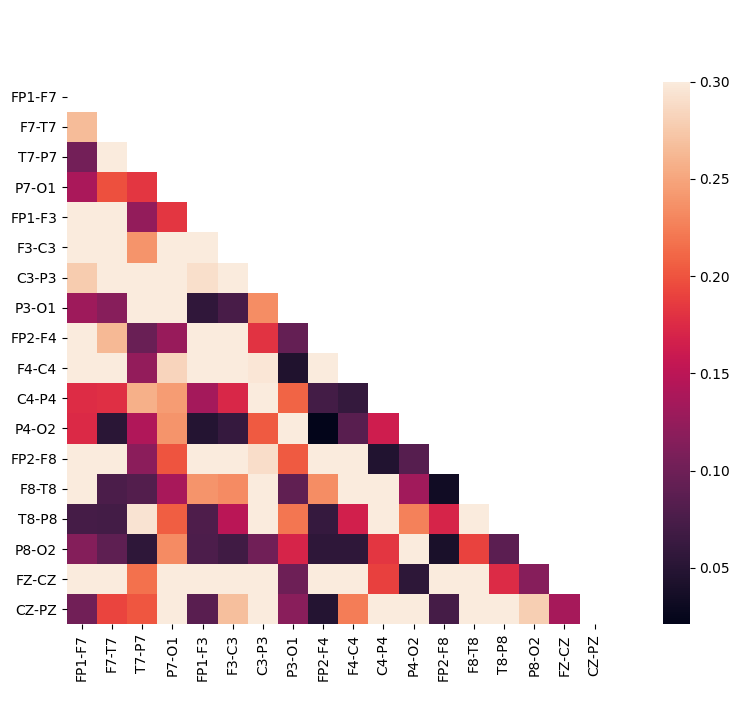
\includegraphics[scale=.4795]{Correlações 5 primeiros segundos 1 paciente}
	\caption{Mapas de calor das correlações cruzadas dos 5 primeiros segundos do primeiro paciente.}
	\label{fig:heatmap}
\end{figure}



Devido aos baixos valores de correlações as conexões entre os nós ficam com baixos pesos e isso implica em um baixo tamanho de caminho característico, excentricidades, raio e diâmetro. Um problema comum em diversos exames de diversos pacientes é que, em certos momentos, os eletrodos acidentalmente soltam da pele do paciente fazendo com que o EEG fique constante tornando as variâncias dos canais nulas impossibilitando o calculo das correlações.

\section*{Conclusões}

O processo de extração de características com base na Teoria de Grafos aqui descrito foi bem sucedido, possibilitando a obtenção de vetores de características para sinais EEG de pacientes do banco de dados Physionet. O ponto negativo dos métodos utilizados neste trabalho é o tempo que demanda para a extração de tais características. Em alguns casos, cada hora de EEG levou 1 hora para ser processado em um notebook, em uma aplicação real em que essa análise será feita em um dispositivo embarcado e em tempo real essa demora pode afetar e muito o uso dos dados aqui obtidos. Portanto, como trabalho futuro, propões-se a investigação de formas de redução desse tempo.

\section*{Agradecimentos}

Os autores agradecem ao CNPq pelo apoio financeiro (Programa Institucional de Bolsas de Iniciação Científica e Tecnológica do Instituto Federal de Educação Ciência e Tecnologia de São Paulo PIBIFSP 2021)

\bibliography{bibliografia.bib}

\end{document}
